\documentclass{article}
\usepackage{tikz}

\begin{document}

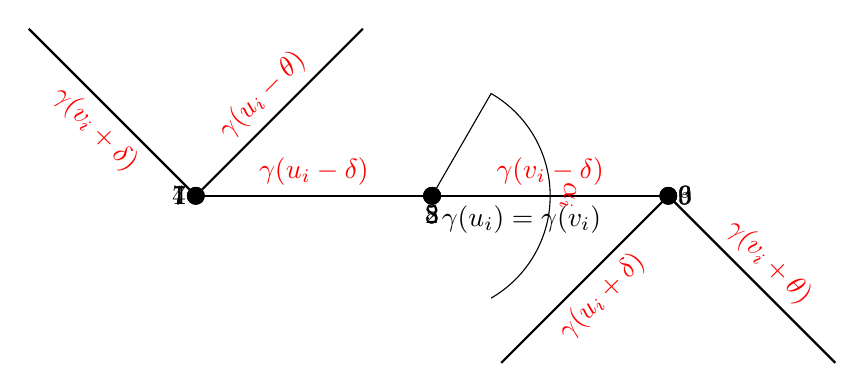
\begin{tikzpicture}[scale=1.5]
    % Define coordinates for the points
    \coordinate (A) at (-2,0);
    \coordinate (B) at (0,0);
    \coordinate (C) at (2,0);
    
    % Draw the main line segments
    \draw[thick] (A) -- (B) node[midway,above,sloped,red] {$\gamma(u_i-\delta)$};
    \draw[thick] (B) -- (C) node[midway,above,sloped,red] {$\gamma(v_i-\delta)$};
    
    % Draw the additional lines and labels
    \draw[thick] (A) -- ++(45:2) node[midway,above,sloped,red] {$\gamma(u_i-\theta)$};
    \draw[thick] (C) -- ++(-45:2) node[midway,above,sloped,red] {$\gamma(v_i+\theta)$};
    \draw[thick] (A) -- ++(135:2) node[midway,below,sloped,red] {$\gamma(v_i+\delta)$};
    \draw[thick] (C) -- ++(-135:2) node[midway,below,sloped,red] {$\gamma(u_i+\delta)$};
    
    % Draw the intersection point and label it
    \filldraw (B) circle (2pt) node[below right] {$\gamma(u_i)=\gamma(v_i)$};
    
    % Draw the angle label
    \draw (B) -- ++(60:1) arc (60:-60:1) node[midway,above,sloped,red] {$\alpha_i$};
    
    % Label the points with numbers
    \filldraw (A) circle (2pt) node[left] {1};
    \filldraw (B) circle (2pt) node[below] {2};
    \filldraw (C) circle (2pt) node[right] {3};
    \filldraw (A) circle (2pt) node[left] {4};
    \filldraw (B) circle (2pt) node[below] {5};
    \filldraw (C) circle (2pt) node[right] {6};
    \filldraw (A) circle (2pt) node[left] {7};
    \filldraw (B) circle (2pt) node[below] {8};
    \filldraw (C) circle (2pt) node[right] {9};
\end{tikzpicture}

\end{document}